\input{header.tex}

\subject{\texorpdfstring{\vspace{2ex}}{}207\texorpdfstring{\vspace{-2ex}}{}} % Nummer
\title{Das Kugelfall\texorpdfstring{\hspace{0.15ex}}{}-\texorpdfstring{\hspace{-0.15ex}}{}Viskosimeter nach Höppler} % Titel
\date{
	Durchführung: 15. Dezember 2022 % Datum
	\\ Abgabe: 7. Januar 2023 % Datum
}

\sisetup{per-mode=reciprocal}
\AtNextBibliography{\scriptsize}

\begin{document}

\pagenumbering{gobble}
\maketitle
\pagenumbering{arabic}

\thispagestyle{empty}
\tableofcontents
\newpage

% Titel: Ziel des Versuchs
% Theorie: Physikalische Grundlagen von Versuch/Messverfahren, Gleichungen ohne Herleitung knapp erklären
\section{Theorie}
\label{sec:theorie}

\subsection{Relaxationsvorgänge}

Allgemein bezeichnen Relaxationserscheinungen das nichtoszillatorische Einstellen des
Gleichgewichtszustandes eines physikalischen Systems. Unter der Annahme, dass sich die
Änderungsrate dabei proportional zur Abweichung von $A(t)$ zum asymptotischen stationären
Endzustand $A_{\raisebox{0.25ex}{\(\scriptscriptstyle{\infty}\)}\!\!}$ verhält, lässt sich die Gleichung
\begin{equation}
	\pfrac{\symup dA}{\symup dt} = c \hspace{0.3ex} (A(t) -
	A_{\raisebox{0.25ex}{$\scriptscriptstyle{\infty}$}\!}) \label{eqn:rate_allgemein}
\end{equation}
mit der Konstante $c$ aufstellen. Integration von \eqref{eqn:rate_allgemein} über die
Zeitpunkte $0$ bis $t$ liefert
\begin{equation}
	\int\limits_{A_0}^{\raisebox{-0.25ex}{$\scriptstyle{A(t)}$}} \!\!
	\pfrac{\symup dA}{\hspace{0.15ex}A - A_{\raisebox{0.25ex}{$\scriptscriptstyle{\infty}$}}} = \!\!
	\int\limits_0^t \! c \, \symup dt' \stepcounter{equation}\tag{2a}
\end{equation}
als entsprechende Operationsvorschrift sowie die äquivalente Formulierung
\begin{equation}
	\ln \pfrac{A(t) - A_{\raisebox{0.25ex}{$\scriptscriptstyle{\infty}$}}}{A_0 -
	A_{\raisebox{0.25ex}{$\scriptscriptstyle{\infty}$}}} = c \hspace{0.15ex} t \tag{2b}
\end{equation}
für deren Ergebnis. Durch Auflösen nach der Größe $A(t)$ ergibt sich damit der Ausdruck
\begin{equation}
	A(t) = A_{\raisebox{0.25ex}{$\scriptscriptstyle{\infty}$}\!} + \hspace{0.15ex}
	(A_0 - A_{\raisebox{0.25ex}{$\scriptscriptstyle{\infty}$}\!}) \hspace{0.15ex}
	\exp (c \hspace{0.15ex} t) \tag{2c} \label{eqn:relax_allgemein}
\end{equation}
zur Beschreibung des Systems. Aus \eqref{eqn:relax_allgemein} folgt noch $c < 0$, sodass $A(t)$
beschränkt ist.

\subsection{Kondensatorladung}

Mit dem Ladungsträgerstrom $I$ und der lokalen Ladung $Q$ gilt die Beziehung
\begin{equation}
	\symup dQ = - I \symup dt
	\label{eqn:ladung}
\end{equation}
an jedem Punkt in der Schaltung. Nach dem ohmschen Gesetz kann außerdem
\begin{equation}
	U \hspace{-0.025ex} = RI
	\label{eqn:ohm}
\end{equation}
geschrieben werden, wobei die Spannung $U$ am Widerstand $R$ abfällt. Daraus folgt dann
\begin{equation}
	U \hspace{-0.025ex} = \pfrac{Q}{C} = RI = -R \,\pfrac{\symup dQ}{\symup dt}
	\stepcounter{equation}\tag{5a}
\end{equation}
als Differentialgleichung am Kondensator der Kapazität $C$. Umgeschrieben in die Form
\begin{equation}
	\pfrac{\symup dQ}{\symup dt} = -\pfrac{1}{RC} \, Q
	\tag{5b}
\end{equation}
entspricht dies nach \eqref{eqn:relax_allgemein} dem Zusammenhang
\begin{equation}
	Q(t) = Q_{\raisebox{0.25ex}{$\scriptscriptstyle{\infty}$}\!} + \hspace{0.15ex}
	(Q_0 - Q_{\raisebox{0.25ex}{$\scriptscriptstyle{\infty}$}\!}) \hspace{0.15ex}
	\exp \! \left(-\pfrac{1}{RC} \, \hspace{0.15ex} t\right)
	\label{eqn:relax_kondensator}
\end{equation}
für den zeitlichen Verlauf der Kondensatorladung.

\subsubsection{Entladevorgang}

Bei der Entladung fällt die anfängliche Ladung $Q_0$ gegen
$Q_{\raisebox{0.25ex}{$\scriptscriptstyle{\infty}$}\!} = 0$ ab. Laut \eqref{eqn:relax_kondensator}
ist dann
\begin{align}
	Q(t) &= Q_0 \exp \! \left(-\pfrac{1}{RC} \, \hspace{0.15ex} t\right)
	\stepcounter{equation}\tag{7a}
	\label{eqn:entladung_ladung} \\
	\intertext{gegeben. Gleichzeitig lässt sich mit $Q = CU$ und $Q_0 = CU_{\hspace{-0.15ex}0}$ der Ausdruck}
	U\hspace{-0.025ex}(t) &= U_{\!0} \exp \! \left(-\pfrac{1}{RC} \, \hspace{0.15ex} t\right)
	\tag{7b}
	\label{eqn:entladung_spannung}
\end{align}
für die Kondensatorspannung aufstellen.

\subsubsection{Aufladevorgang}

Anders als zuvor ist der Kondensator mit $Q_0 = 0$ zunächst entladen. Unter der angelegten
Gleichspannung $U_{\hspace{-0.15ex}0}$ gilt
$Q_{\raisebox{0.25ex}{$\scriptscriptstyle{\infty}$}\!} = CU_{\hspace{-0.15ex}0}$ als aufgeladener Endzustand.
Einsetzen in \eqref{eqn:relax_kondensator} liefert
\begin{align}
	Q(t) &= CU_{\hspace{-0.15ex}0} 
	\!\left(\!1 - \exp \! \left(-\pfrac{1}{RC} \, \hspace{0.15ex} t\right) \!\right)
	\stepcounter{equation}\tag{8a}
	\label{eqn:aufladung_ladung} \\
	\intertext{zur Beschreibung der Ladung. Weiter definiert der Term}
	U\hspace{-0.025ex}(t) &= U_{\!0}
	\!\left(\!1 - \exp \! \left(-\pfrac{1}{RC} \, \hspace{0.15ex} t\right) \!\right)
	\tag{8b}
	\label{eqn:aufladung_spannung}
\end{align}
den entsprechenden Spannungsverlauf.

\subsubsection{Zeitkonstante}

Mit $\tau = RC$ ist die charakteristische Zeitkonstante des RC\hspace{0.15ex}-Kreises bezeichnet.
Diese bemisst die Geschwindigkeit, mit welcher das System gegen den Endzustand strebt.

\newpage

\subsection{Periodische Auslenkung}

Wird nun stattdessen eine periodische Generatorspannung der Gestalt
$U_{\hspace{-0.025ex}\text{in}\!} = U_{\hspace{-0.025ex}0} \cos(\omega t)$ mit einer Kreisfrequenz
$\omega = 2\pi \hspace{0.15ex} \nu$ angelegt, bietet sich die Durchführung einer komplexen
Wechselstromrechnung an.

\subsubsection{Impedanzen}

Mit der imaginären Einheit $i \mkern1mu$ kann die Gesamtimpedanz der Schaltung als
\begin{equation}
	Z_{\hspace{-0.15ex}RC} = Z_{\hspace{-0.15ex}R} + Z_C = R + \pfrac{1}{i \mkern1mu \omega \hspace{0.15ex} C}
	\label{eqn:impedanz}
\end{equation}
zusammengefasst werden. Dabei entspricht der reale Term $Z_{\hspace{-0.15ex}R}$ dem verbauten ohmschen
Wirkwiderstand. Der Blindwiderstand des Kondensators ist mit $Z_C$ \mbox{angegeben. Weiter gilt}
\begin{equation}
	U \hspace{-0.025ex} = ZI
	\label{eqn:ohm_komplex}
\end{equation}
als verallgemeinerter Zusammenhang zwischen Spannung, Impedanz und Stromstärke. Speziell folgen
aus \eqref{eqn:ohm_komplex} die Proportionalitäten
$U_{\hspace{-0.025ex}\text{in}\!} \propto Z_{\hspace{-0.15ex}RC}\hspace{0.15ex}$ für die
Eingangsspannung und $U_{\hspace{-0.025ex}\text{out}\!} \propto Z_C\hspace{0.15ex}$ für jene Spannung,
die am Kondensator abfällt. Durch \eqref{eqn:impedanz} lässt sich mit
\begin{equation}
	H = \pfrac{U_{\hspace{-0.025ex}\text{out}}}{U_{\hspace{-0.025ex}\text{in}\!}} = 
	\pfrac{Z_C}{Z_{\hspace{-0.15ex}RC}} = \pfrac{1}{1 + i \mkern1mu \omega R \hspace{0.15ex} C}
	\label{eqn:transmission}
\end{equation}
schließlich das Übertragungsverhältnis aufstellen. 

\subsubsection{Amplitudenverlauf}

Aus Gleichung \eqref{eqn:transmission} ist die betragsmäßige Transmission direkt mit dem Ausdruck
\begin{equation}
	\left|H\hspace{0.2ex}\right| =
	\left|\pfrac{U_{\hspace{-0.025ex}\text{out}}}{U_{\hspace{-0.025ex}\text{in}\!}}\right| = 
	\pfrac{\left|Z_C\right|}{\left|Z_{\hspace{-0.15ex}RC}\right|} =
	\pfrac{1}{\sqrt{1 + \omega^2 \hspace{-0.2ex} R^2 C^2}}
\end{equation}
bestimmt. Die Amplitude $U\hspace{-0.025ex}$ der Kondensatorspannung verläuft dann nach der \mbox{Beziehung}
\begin{equation}
	U\hspace{-0.025ex}(\omega) = \pfrac{U_{\hspace{-0.025ex}0}}{\sqrt{1 + \omega^2 \hspace{-0.2ex} R^2 C^2}}
	\label{eqn:amplitude_frequenz}
\end{equation}
in Abhängigkeit zur Kreisfrequenz $\omega$. Demnach bildet der RC\hspace{0.15ex}-Kreis einen Tiefpass.

\subsubsection{Phasenverschiebung}

Konjugiertes Ergänzen von \eqref{eqn:transmission} zeigt, dass zusätzlich die Proportionalitätsrelation
\begin{equation}
	H \hspace{-0.15ex} \propto 1 - \hspace{0.15ex} i \mkern1mu \omega R \hspace{0.15ex} C
	\label{eqn:proportion}
\end{equation}
erfüllt ist. Indem aus der Gaußschen Zahlenebene der geometrische Zusammenhang
\begin{equation}
	\tan(\varphi) = \pfrac{\sin(\varphi)}{\cos(\varphi)}
	= \pfrac{\operatorname{Im}(\hspace{-0.1ex}H\hspace{0.1ex})}{\operatorname{Re}(\hspace{-0.1ex}H\hspace{0.1ex})}
	= - \hspace{0.15ex} \omega R \hspace{0.15ex} C
	\label{eqn:phase_tangens}
\end{equation}
entnommen wird, lässt sich so die Phase $\varphi = \operatorname{arg}(\hspace{-0.1ex}H\hspace{0.1ex})$
zwischen $U_{\hspace{-0.025ex}\text{in}\!}$ und $U_{\hspace{-0.025ex}\text{out}\!}$ als
\begin{equation}
	\varphi(\omega) = - \arctan ( \omega R \hspace{0.15ex} C \hspace{0.1ex})
	\label{eqn:phase}
\end{equation}
definieren. Schließlich folgt nach Einsetzen von \eqref{eqn:phase_tangens} in \eqref{eqn:amplitude_frequenz} noch
\begin{equation}
	U\hspace{-0.025ex}(\varphi) = \pfrac{\cos(\varphi)}{\sqrt{\cos^2(\varphi) + \sin^2(\varphi)}}
	\, U_{\hspace{-0.025ex}0} = \cos(\varphi) \, U_{\hspace{-0.025ex}0}
	\label{eqn:amplitude_phase}
\end{equation}
als phasenabhängiger Ausdruck für die Amplitudenspannung. 

\subsection{Integrationsanwendung}

Bei Eingangsspannungen mit $\omega \gg \tau^{-1}$ läuft $Z_C$ gegen Null. Dann kann die Näherung
\begin{equation}
	U_{\hspace{-0.025ex}\text{in}\!} = ZI = Z_{\hspace{-0.15ex}R} I = RI = R \, \pfrac{\symup dQ}{\symup dt} =
	RC \: \pfrac{\symup dU_{\hspace{-0.025ex}\text{out}\!}}{\symup dt}
	\stepcounter{equation}\tag{18a}
\end{equation}
aus \eqref{eqn:ohm_komplex} hergeleitet werden. Integrieren von $0$ bis $t$ liefert die Beziehung
\begin{equation}
	U_{\hspace{-0.025ex}\text{out}\!}= \pfrac{1}{\hspace{-0.15ex}RC\hspace{0.15ex}} \!
	\int\limits_0^t \! U_{\hspace{-0.025ex}\text{in}\!} \: \symup dt'
	\tag{18b}
	\label{eqn:integral}
\end{equation}
für den RC\hspace{0.15ex}-Kreis. Dieser beschreibt somit einen Integrator hochfrequenter Signale.

\newpage

\subsection{Fehlerrechnung}

Um die Abweichung der Messgrößen zu untersuchen, werden noch einige weitere Formeln benötigt.
Die Rechenvorschrift für den Mittelwert $\overline{x}$ ist mit
\begin{equation}
	\overline{x} = \pfrac{1}{N \,} \sum_{n=1}^N x_n
	\label{eqn:mittel}
\end{equation}
gegeben. Zur Bestimmung der Standardabweichung $\symup{\Delta}\overline{x}$ kann
\begin{equation}
	(\symup{\Delta}\overline{x})^2 = \pfrac{1}{N(N-1)} \sum_{n=1}^N (x_n \! - \overline{x})^2
	\label{eqn:std}
\end{equation}
verwendet werden. Durch die Gaußsche Fehlerfortpflanzung
\begin{equation}
	(\symup{\Delta}f)^2 = \sum_{n=1}^N
	\left( \! \pfrac{\partial^{\!} f}{\partial x_{\raisebox{0.2ex}{$\scriptstyle{n}$}}} \!
	\right)^{\!\! 2} \!\! (\symup{\Delta}x_{\raisebox{0.2ex}{$\scriptstyle{n}$}})^2
	\label{eqn:gauss}
\end{equation}
ist die Abweichung $\symup{\Delta}f$ für von fehlerbehafteten Werten $x_n \!$ abhängige
Größen $\hspace{-0.2ex} f \hspace{0.2ex}$ definiert.

\subsection{Lineare Regression}

Entlang der linear abhängigen Messgrößen $(x_n,y_n)$ für $n = 1,\dotsc,\hspace{-0.1ex}N\hspace{0.1ex}$
lassen sich über
\begin{align}
	m = \pfrac{\overline{x\hspace{0.15ex}y\hspace{0.15ex}} - \overline{x} \: \overline{y\hspace{0.15ex}}}
	{\overline{x^2} - \overline{x}^{\hspace{0.15ex}2}} && b = \overline{y\hspace{0.15ex}} - m \overline{x}
	\label{eqn:regression}
\end{align}
die Parameter der Ausgleichsgerade $y = mx + b$ berechnen.

% Aufgabe: Messaufgaben auflisten
% Vorbereitung: Vorbereitungsaufgaben bearbeiten
% Versuchsaufbau: Verwendete Apparatur, Beschreibung Funktionsweise/Nutzen mit Skizze/Foto

\vfill

\section{Aufgabe}
Zielsetzung dieser Versuchsreihe ist die Untersuchung des Verhaltens eines RC\hspace{0.15ex}-Kreises
in Abhängigkeit von Zeit, Frequenz und Phase. Speziell soll anhand der beobachteten Beziehungen
die Zeitkonstante $\tau$ bestimmt werden. Dazu werden entsprechende Messungen durchgeführt und
aufbauend auf den theoretischen Grundlagen ausgewertet.

\newpage

\section{Durchführung}
\label{sec:durchführung}

\begin{figure}
	\centering
	\vspace{1.23ex}
	\resizebox{0.93\width}{!}{\begin{tikzpicture}\tikzstyle{every node} = [font = \small]

\ctikzset{bipoles/thickness = 1}
\ctikzset{bipoles/length = 1cm}

\begin{scope}[line width = 1pt]
	% Frequenzmesser
	\draw
		(0,-1) to[short]
		++(-3,0) to[rmeter, t=\raisebox{-0.6ex}{$\hspace{-0.1ex}\small\nu$}]
		++(0,4) to[short]
		++(3,0);

	% Funktionsgenerator
	\draw
		(0,-1) to[short, *-o] ++(0,0.55);
	\draw
		(-0.2,-0.25) to[short, o-]
		++(0,0.2) to[short]
		++(-0.55,0) to[sV]
		++(0,1) to[short]
		++(0.55,0) to[short, -o]
		++(0,0.2);
	\draw
		(0,-0.25) to[tV, o-o] ++(0,1.4);
	\draw
		(0.2,-0.25) to[short, o-]
		++(0,0.2) to[short]
		++(0.55,0) to[sqV]
		++(0,1) to[short]
		++(-0.55,0) to[short, -o]
		++(0,0.2);
	\draw
		(0,1.35) to[R, o-, l=$R_0$]
		++(0,1.4) to[short, -*]
		++(0,0.25);
	
	% RC-Glied
	\draw
		(0,3) to[R, -*, l_=$R$]
		++(3,0) to[C, -*, l_=\raisebox{-0.2ex}{$C$}]
		++(0,-4) to[short]
		++(-3,0);

	% Oszillograph
	\draw
		(3,3) to[short]
		++(3,0) to[short]
		++(0,-1.7);
	\draw
		(5.85,1.3) -- ++(0.3,0);
	\draw
		(5.85,0.7) -- ++(0.3,0);
	\draw
		(6,0.7) to[short, -*]
		++(0,-1.7) -- ++(0,-0.3);
	\draw
		(5.8,-1.3) -- ++(0.4,0);
	\draw
		(5.865,-1.375) -- ++(0.27,0);
	\draw
		(5.925,-1.45) -- ++(0.15,0);
	\draw
		(0,3) to[short]
		++(0,0.75) to[short]
		++(6.75,0) to[short]
		++(0,-2.45);
	\draw
		(6.6,1.3) -- ++(0.3,0);
	\draw
		(6.6,0.7) -- ++(0.3,0);
	\draw
		(6.75,0.7) to[short]
		++(0,-1.7) to[short]
		++(-3.75,0);
	\draw
		(5.125,-1) to[short, *-]
		++(0,2) to[short]
		++(0.5,0);
	\draw
		(5.625,0.85) -- ++(0,0.3);
	\draw
		(7.125,0.85) -- ++(0,0.3);
	\draw
		(7.125,1) to[short, -*]
		++(0.5,0);
	\draw[rounded corners=3mm]
		(5.525,1.4) -- ++(1.7,0) -- ++(0,-0.8) -- ++(-1.7,0) -- cycle;

	\node at (5.5,1.7) {CH\hspace{0.3ex}1};
	\node at (7.25,1.7) {CH\hspace{0.3ex}2};

	\node[rotate=270] at (8,1) {Oszillograph};
	\node[rotate=90] at (-3.6,1) {Frequenzmesser};
	\node at (0,-1.325) {Funktionsgenerator};
\end{scope}
\end{tikzpicture}}
	\vspace{1.23ex}
	\caption{Veranschaulichendes Schaltbild des Messaufbaus.}
	\label{fig:circuit}
\end{figure}

Zunächst soll der Entladungsvorgang des Kondensators nach \eqref{eqn:entladung_spannung} betrachtet werden.
Am Funktionsgenerator in Abbildung \ref{fig:circuit} wird dazu ein Rechtecksignal eingestellt. Durch Wahl
einer ausreichend großen Periode $T \gg \tau$ fällt die Kondensatorspannung am Eingang \mbox{CH\hspace{0.3ex}1}
gegen Null ab. Auf diesem Weg lässt sich die Messskala kalibrieren. Anschließend wird unter erhöhter Frequenz
ein Druck des Oszilloskopschirms angefertigt, um aus den vom Verlauf abzulesenden Daten die Zeitkonstante
$\tau$ zu bestimmen. Im Weiteren erlaubt das Abgreifen einer veränderlichen Sinusspannung, über das
\mbox{Transmissionsverhalten~\eqref{eqn:transmission} auf} $\tau = RC$ zu schließen. Die Amplitude der
Kondensatorspannung wird hierbei mit den entsprechenden Frequenzen nachgehalten. Darauf folgend ist die
Phasenabhängigkeit~\eqref{eqn:phase} zu untersuchen. Es werden Verlauf von Eingangsspannung
an CH\hspace{0.3ex}2 und Ausgangsspannung an CH\hspace{0.3ex}1 gemeinsam betrachtet, um daraus die
Verschiebung
\begin{equation}
	\varphi = \pfrac{a}{b} \, \qty{360}{\degree}
\end{equation}
mit den Größen $a$ und $b$ nach Abbildung \ref{fig:ab} zu erhalten. 

\begin{figure}
	\centering
	\vspace{0.615ex}
	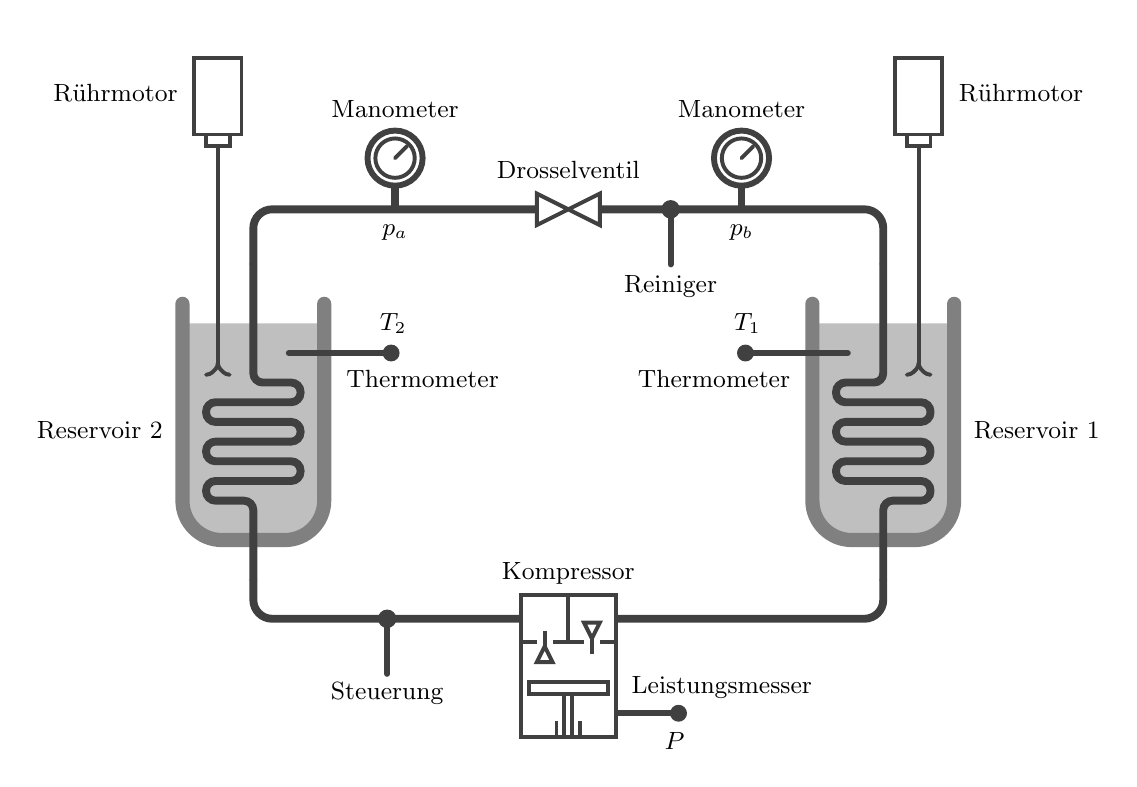
\begin{tikzpicture}
		\tikzstyle{every node} = [font = \small]

% frame
\draw[draw=white] 
	(0,0) -- ++(0,9) -- ++(8,0) -- ++(0,-9) -- cycle;

% valve
\draw[draw=darkgray, line width=0.5mm] 
	(3.6,6.7) -- ++(0,-0.2) -- ++(0.8,0.4) -- ++(0,-0.4) -- ++(-0.8,0.4) -- cycle;

% compresser
\draw[draw=darkgray, line width=0.5mm] 
	(3.4,0) -- ++(0,1.8) -- ++(1.2,0) -- ++(0,-1.8) -- cycle;
\draw[draw=darkgray, line width=0.5mm] 
	(4,1.8) -- ++(0,-0.6);
\draw[draw=darkgray, line width=0.5mm] 
	(3.8,1.2) -- ++(0.4,0);
\draw[draw=darkgray, line width=0.5mm] 
	(3.4,1.2) -- ++(0.2,0);
\draw[draw=darkgray, line width=0.5mm] 
	(4.6,1.2) -- ++(-0.2,0);
\draw[draw=darkgray, line width=0.5mm] 
	(3.7,1.35) -- ++(0,-0.2);
\draw[draw=darkgray, line width=0.5mm] 
	(3.7,1.15) -- ++(-0.1,-0.2) -- ++(0.2,0) -- cycle;
\draw[draw=darkgray, line width=0.5mm] 
	(4.3,1.25) -- ++(0,-0.2);
\draw[draw=darkgray, line width=0.5mm] 
	(4.3,1.25) -- ++(-0.1,0.2) -- ++(0.2,0) -- cycle;
\draw[draw=darkgray, line width=0.5mm] 
	(3.5,0.7) -- ++(1,0) -- ++(0,-0.15) -- ++(-1,0) -- cycle;
\draw[draw=darkgray, line width=0.5mm] 
	(3.95,0.55) -- ++(0,-0.55);
\draw[draw=darkgray, line width=0.5mm] 
	(4.05,0.55) -- ++(0,-0.55);
\draw[draw=darkgray, line width=0.5mm] 
	(3.85,0.2) -- ++(0,-0.2);
\draw[draw=darkgray, line width=0.5mm] 
	(4.15,0.2) -- ++(0,-0.2);

% wattmeter
\draw[draw=darkgray, line width=0.75mm] 
	(4.6,0.3) -- (5.4,0.3);
\draw[draw=darkgray, fill=darkgray] 
	(5.4,0.3) circle (1mm);

% control
\draw[draw=darkgray, line width=0.75mm, line cap=round] 
	(1.7,1.5) -- (1.7,0.8);
\draw[draw=darkgray, fill=darkgray] 
	(1.7,1.5) circle (1.1mm);

% diffuser
\draw[draw=darkgray, line width=0.75mm, line cap=round] 
	(5.3,6.7) -- (5.3,6);
\draw[draw=darkgray, fill=darkgray] 
	(5.3,6.7) circle (1.1mm);

% left

% bucket
\draw[draw=lightgray, fill=lightgray, line width=0mm, line cap=round, rounded corners=5mm] 
	(-0.9,5.25) -- ++(0,-2.75) -- ++(1.8,0) -- ++(0,2.75);
\draw[draw=gray, line width=1.8mm, line cap=round, rounded corners=5mm] 
	(-0.9,5.5) -- ++(0,-3) -- ++(1.8,0) -- ++(0,3);
% mixer
\draw[draw=darkgray, line width=0.5mm] 
	(-0.45,7.5) -- ++(0,-2.75);
\draw[draw=darkgray, line width=0.5mm, line cap=round, rounded corners=0.45mm] 
	(-0.45,4.75) -- ++(0,-0.05) -- ++(-0.1,-0.1) -- ++(-0.05,0);
\draw[draw=darkgray, line width=0.5mm, line cap=round, rounded corners=0.45mm] 
	(-0.45,4.75) -- ++(0,-0.05) -- ++(0.1,-0.1) -- ++(0.05,0);
\draw[draw=darkgray, line width=0.5mm] 
	(-0.6,7.65) -- ++(0,-0.15) -- ++(0.3,0) -- ++(0,0.15);
\draw[draw=darkgray, line width=0.5mm] 
	(-0.75,7.65) -- ++(0.6,0) -- ++(0,0.975) -- ++(-0.6,0) -- cycle;
% thermometer
\draw[draw=darkgray, line width=0.75mm, line cap=round] 
	(0.45,4.875) -- (1.75,4.875);
\draw[draw=darkgray, fill=darkgray] 
	(1.75,4.875) circle (1mm);
% manometer
\draw[draw=darkgray, line width=1mm] 
	(1.8,6.7) -- (1.8,7);
\draw[draw=darkgray, line width=0.75mm] 
	(1.8,7.35) circle (3.5mm);
\draw[draw=darkgray, line width=0.5mm] 
	(1.8,7.35) circle (2.5mm);
\draw[draw=darkgray, line width=0.5mm, line cap=round] 
	(1.8,7.35) -- ++(0.15,0.15);
% snake
\draw[draw=darkgray, line width=1mm, line cap=round, rounded corners=1.2mm] 
	(0,6) -- ++(0,-1.5) -- ++(0.6,0) -- ++(0,-0.25) -- ++(-1.2,0) -- ++(0,-0.25)
	-- ++(1.2,0) -- ++(0,-0.25) -- ++(-1.2,0) -- ++(0,-0.25)
	-- ++(1.2,0) -- ++(0,-0.25) -- ++(-1.2,0) -- ++(0,-0.25)
	-- ++(0.6,0) -- (0,2);
\draw[draw=darkgray, line width=1mm, rounded corners=2.4mm] 
	(0,2) -- (0,1.5) -- (3.4,1.5);
\draw[draw=darkgray, line width=1mm, rounded corners=2.4mm] 
	(0,6) -- (0,6.7) -- (3.6,6.7);

% right

% bucket
\draw[draw=lightgray, fill=lightgray, line width=0mm, line cap=round, rounded corners=5mm] 
	(7.1,5.25) -- ++(0,-2.75) -- ++(1.8,0) -- ++(0,2.75);
\draw[draw=gray, line width=1.8mm, line cap=round, rounded corners=5mm] 
	(7.1,5.5) -- ++(0,-3) -- ++(1.8,0) -- ++(0,3);
% mixer
\draw[draw=darkgray, line width=0.5mm] 
	(8.45,7.5) -- ++(0,-2.75);
\draw[draw=darkgray, line width=0.5mm, line cap=round, rounded corners=0.45mm] 
	(8.45,4.75) -- ++(0,-0.05) -- ++(-0.1,-0.1) -- ++(-0.05,0);
\draw[draw=darkgray, line width=0.5mm, line cap=round, rounded corners=0.45mm] 
	(8.45,4.75) -- ++(0,-0.05) -- ++(0.1,-0.1) -- ++(0.05,0);
\draw[draw=darkgray, line width=0.5mm] 
	(8.3,7.65) -- ++(0,-0.15) -- ++(0.3,0) -- ++(0,0.15);
\draw[draw=darkgray, line width=0.5mm] 
	(8.15,7.65) -- ++(0.6,0) -- ++(0,0.975) -- ++(-0.6,0) -- cycle;
% thermometer
\draw[draw=darkgray, line width=0.75mm, line cap=round] 
	(7.55,4.875) -- (6.25,4.875);
\draw[draw=darkgray, fill=darkgray] 
	(6.25,4.875) circle (1mm);
% manometer
\draw[draw=darkgray, line width=1mm] 
	(6.2,6.7) -- (6.2,7);
\draw[draw=darkgray, line width=0.75mm] 
	(6.2,7.35) circle (3.5mm);
\draw[draw=darkgray, line width=0.5mm] 
	(6.2,7.35) circle (2.5mm);
\draw[draw=darkgray, line width=0.5mm, line cap=round] 
	(6.2,7.35) -- ++(0.15,0.15);
% snake
\draw[draw=darkgray, line width=1mm, line cap=round, rounded corners=1.2mm] 
	(8,6) -- ++(0,-1.5) -- ++(-0.6,0) -- ++(0,-0.25) -- ++(1.2,0) -- ++(0,-0.25)
	-- ++(-1.2,0) -- ++(0,-0.25) -- ++(1.2,0) -- ++(0,-0.25)
	-- ++(-1.2,0) -- ++(0,-0.25) -- ++(1.2,0) -- ++(0,-0.25)
	-- ++(-0.6,0) -- (8,2);
\draw[draw=darkgray, line width=1mm, rounded corners=2.4mm] 
	(8,2) -- (8,1.5) -- (4.6,1.5);
\draw[draw=darkgray, line width=1mm, rounded corners=2.4mm] 
	(8,6) -- (8,6.7) -- (4.4,6.7);

% labels
\node at (-1.75,8.175) {Rührmotor};
\node at (9.75,8.175) {Rührmotor};
\node at (1.8,7.975) {Manometer};
\node at (6.2,7.975) {Manometer};
\node at (4,7.2) {Drosselventil};
\node at (1.8,6.4) {$p_a$};
\node at (6.2,6.4) {$p_b$};
\node at (5.3,5.725) {Reiniger};
\node at (1.775,5.25) {$T_2$};
\node at (6.275,5.25) {$T_1$};
\node at (2.15,4.55) {Thermometer};
\node at (5.85,4.55) {Thermometer};
\node at (-1.95,3.9) {Reservoir $2$};
\node at (9.95,3.9) {Reservoir $1$};
\node at (4,2.075) {Kompressor};
\node at (1.7,0.55) {Steuerung};
\node at (5.95,0.625) {Leistungsmesser};
\node at (5.35,-0.05) {$P$};

	\end{tikzpicture}
	\vspace{1.23ex}
	\caption{Schematische Darstellung des Oszillographenschirms.}
	\label{fig:ab}
\end{figure}

Anhand der so gewonnenen Messwerte wird zur Phase auch eine Polarprojektion des Zusammenhangs
\eqref{eqn:amplitude_phase} vorgenommen. Zuletzt ist noch die Integralfunktion des
RC\hspace{0.15ex}-Gliedes qualitativ anhand verschiedener Signaltypen abgebildet.

% Messwerte: Alle gemessenen Größen tabellarisch darstellen
% Auswertung: Berechnung geforderter Ergebnisse mit Schritten/Fehlerformeln/Erläuterung/Grafik (Programme)
\section{Auswertung}
\label{sec:auswertung}

Die hier verwendeten Komponenten weisen baubedingt gewisse Toleranzbereiche sowie unsystematische Fehler auf.
Diese sind in relativer Darstellung angegeben, können für die Fehlerfortpflanzung also direkt als Verhältnis
in~\eqref{eqn:speziell} eingesetzt werden. Außerdem folgt aufgrund der Funktionsweise des Potentiometers
für Versuche, in denen ein solches zur Einstellung eines Widerstandsverhältnisses gebraucht wird:
\begin{equation*}
	\pfrac{\vphantom{\int}R_3}{\vphantom{\int}R_4} =
	\pfrac{\vphantom{\int}R_3}{\vphantom{\int} \qty{1}{\kilo\ohm} - \! R_3}
\end{equation*}
Zur Bestimmung der Abweichung wird jeweils die Standardabweichung des Mittelwertes nach~\eqref{eqn:std}
gebildet und mit dem Ergebnis der Fehlerfortpflanzung~\eqref{eqn:gauss} verglichen. Der größere Wert
wird dann als Unsicherheit festgelegt. Zur graphischen Darstellung sowie zum automatisierten Ausgeben
der Tabellen werden die Bibliotheken NumPy \cite{numpy} und Matplotlib \cite{matplotlib}
unter Python \cite{python} genutzt.

\subsection{Wheatstonesche Messbrücke}

\begin{table}
	\centering
	\caption{Messdaten zur Bestimmung ohmscher Widerstände unter Anwendung der
			 Wheatstoneschen Brücke bei $R_4 = \qty{1}{\kilo\ohm} - R_3$.}
		\begin{tabular}
		{S[table-format=4.0]
		 S[table-format=3.0]
		 S[table-format=3.3] 
		 S[table-format=3.0]
		 S[table-format=3.3]}
		\toprule
		& \multicolumn{2}{c}{Wert 13} & \multicolumn{2}{c}{Wert 14} \\
		\cmidrule(lr){2-3} \cmidrule(lr){4-5}
		{$R_2 \mathbin{/} \unit{\ohm}$} &
		{$R_3 \mathbin{/} \unit{\ohm}$} &
		{$R_x \mathbin{/} \unit{\ohm}$} &
		{$R_3 \mathbin{/} \unit{\ohm}$} &
		{$R_x \mathbin{/} \unit{\ohm}$} \\
		\midrule
		 500 & 391 & 321.018 & 645 & 908.451 \\
		 664 & 326 & 321.163 & 577 & 905.740 \\
		1000 & 243 & 321.004 & 475 & 904.762 \\
		\bottomrule
	\end{tabular}

	\label{tab:ohm}
\end{table}

Die relative Abweichung für $R_2$ ist mit $\qty{0.2}{\percent}$ angegeben, das am Potentiometer erzeugte
Verhältnis von $R_3$ zu $R_4$ besitzt mit $\qty{0.5}{\percent}$ eine etwas größere Ungenauigkeit. $R_x$
berechnet sich nach Formel~\eqref{eqn:wheatstone}. Daraus und aus den in Tabelle \ref{tab:ohm}
nachgehaltenen Messergebnissen ergeben sich die Mittelwerte mit ihren baubedingten absoluten Fehlern: 
\begin{align*}
	R_{x,13} = \qty{321.1(1.7)}{\ohm} &&
	R_{x,14} = \qty{906.3(4.9)}{\ohm}
\end{align*}
Die Abweichungen der Mittelwerte fallen mit $\symup{\Delta}R_{x,13} = \qty{0.1}{\ohm}$ 
und $\symup{\Delta}R_{x,14} = \qty{1.1}{\ohm}$ deutlich geringer aus. \newpage

\subsection{Kapazitätsmessbrücke}

\begin{table}
	\centering
	\caption{Messdaten zur Bestimmung von Kapazität und Verlustwiderstand.}
		\begin{tabular}
		{S[table-format=3.0]
		 S[table-format=3.0]
		 S[table-format=3.0]
		 S[table-format=3.3]
		 S[table-format=3.3]}
		\toprule
		{$C_2 \mathbin{/} \unit{\nano\farad}$} &
		{$R_2 \mathbin{/} \unit{\ohm}$} &
		{$R_3 \mathbin{/} \unit{\ohm}$} &
		{$C_x \mathbin{/} \unit{\nano\farad}$} &
		{$R_x \mathbin{/} \unit{\ohm}$} \\
		\midrule \\[-1.5ex]
		& \multicolumn{4}{c}{Wert 8} \\
		\cmidrule(lr){2-5}
		450 & 380 & 606 &  292.574 & 584.467 \\
		597 & 288 & 671 &  292.717 & 587.380 \\[1.5ex]
		& \multicolumn{4}{c}{Wert 3 mit Wert 13} \\
		\cmidrule(lr){2-5}
		450 & 412 & 484 &  479.752 & 386.450 \\
		597 & 232 & 589 &  416.582 & 332.477 \\[1.5ex]
		& \multicolumn{4}{c}{Wert 4 mit Wert 13} \\
		\cmidrule(lr){2-5}
		450 & 694 & 321 &  951.869 & 328.091 \\
		597 & 615 & 350 & 1108.714 & 331.154 \\
		\bottomrule
	\end{tabular}

	\label{tab:kapazität}
\end{table}

Der relative Fehler von $C_2$ beträgt $\qty{0.2}{\percent}$, während das Verhältnis von $R_3$ zu $R_4$
weiterhin mit einer Abweichung von $\qty{0.5}{\percent}$ behaftet ist. Um den verstellbaren Widerstand
$R_2$ zu realisieren, wird ein einzelner Ausgang eines Potentiometers genutzt. Der zugehörige Fehler ist
mit $\qty{3}{\percent}$ gegeben. Zur Messung der Kapazitäten werden sie mit Wert 13 {in} Reihe geschaltet.
Dies ermöglicht es, die Verlustwiderstände mit den vorherigen Ergebnissen zu vergleichen. Unter Verwendung
von~\eqref{eqn:kapazität} lassen sich die in Tabelle \ref{tab:kapazität} eingetragenen Messungen auswerten.

Für Wert 4 ergibt sich ein Fehler von $\qty{5.5}{\nano\farad}$, welchen die Standardabweichung
eindeutig übertrifft. Dagegen ist für den kombinierten Verlustwiderstand die Abweichung des Mittelwertes
mit $\symup{\Delta} R_{x,4} = \qty{1.5}{\ohm}$ geringer:
\begin{align*}
	C_{x,4} = \qty{1030(78)}{\nano\farad} && R_{x,4} = \qty{330(10)}{\ohm}
\end{align*}
Zu Wert 3 liegen beide baubedingten Fehler mit $\qty{2.4}{\nano\farad}$ und $\qty{11}{\ohm}$ deutlich
unter ihren entsprechenden Mittelwertsabweichungen:
\begin{align*}
	C_{x,3} = \qty{448(32)}{\nano\farad} &&
	R_{x,3} = \qty{359(27)}{\ohm}
\end{align*}
Der Vergleich der kombinierten Wirkwiderstände mit dem einzelnen zuvor gemessenen Bauteil
$R_{x,13} = \qty{321.1(1.7)}{\ohm}$ zeigt, dass die realen Kondensatoren tatsächlich geringere Verluste
aufweisen, diese aber nicht unbedingt völlig vernachlässigbar sind. 

Für die $RC$-Kombination Wert 8 sind die Messungen ähnlicher, die Standardabweichungen 
$\symup{\Delta} C_{x,8} = \qty{0.1}{\nano\farad}$ und $\symup{\Delta} R_{x,8}= \qty{1.5}{\ohm}$
fallen geringer als die baubedingten Fehler aus:
\begin{align*}
	C_{x,8} = \qty{292.6(1.6)}{\nano\farad} &&
	R_{x,8} = \qty{586(18)}{\ohm}
\end{align*}

\subsection{Induktivitätsmessbrücke}
\label{sec:4.3}

\begin{table}
	\centering
	\caption{Messdaten zur Bestimmung von Induktivität und Verlustwiderstand.}
		\begin{tabular}
		{S[table-format=2.1]
		 S[table-format=2.0]
		 S[table-format=3.0]
		 S[table-format=3.2]
		 S[table-format=3.2]}
		\toprule
		\multicolumn{5}{c}{Wert 18} \\
		\cmidrule(lr){1-5}
		{$L_2 \mathbin{/} \unit{\milli\henry}$} &
		{$R_2 \mathbin{/} \unit{\ohm}$} &
		{$R_3 \mathbin{/} \unit{\ohm}$} &
		{$L_x \mathbin{/} \unit{\milli\henry}$} &
		{$R_x \mathbin{/} \unit{\ohm}$} \\
		\midrule
		20.1 & 24 & 849 & 113.01 & 134.94 \\
		14.6 & 26 & 895 & 124.45 & 221.62 \\
		\bottomrule
	\end{tabular}

	\label{tab:induktivität}
\end{table}

Die Induktivität $L_2$ besitzt eine relative Abweichung \qty{0.2}{\percent}. Für Größen, \mbox{welche ohmsche}
Widerstände enthalten, gelten die gleichen Ungenauigkeiten wie vorher. Werden die
Ausdrücke~\eqref{eqn:induktivität} auf die Messergebnisse aus Tabelle \ref{tab:induktivität} angewendet,
überwiegt erneut die Mittelwertsabweichung im Vergleich zu den baubedingten Fehlern $\qty{0.7}{\milli\henry}$
und $\qty{5.4}{\ohm}$:
\begin{align*}
	L_{x,18} = \qty{118.7(5.7)}{\milli\henry} && R_{x,18} = \qty{178(43)}{\ohm}
\end{align*}

\subsection{Maxwell-Brücke}
\label{sec:4.4}

\begin{table}
	\centering
	\caption{Messdaten zur Bestimmung von Induktivität und Verlustwiderstand mittels der
			 Maxwell-Brücke bei $R_2 = \qty{1}{\kilo\ohm}$.}
		\begin{tabular}
		{S[table-format=3.0]
		 S[table-format=3.0]
		 S[table-format=3.0]
		 S[table-format=3.3]
		 S[table-format=3.3]}
		\toprule
		\multicolumn{5}{c}{Wert 16} \\
		\cmidrule(lr){1-5}
		{$C_4 \mathbin{/} \unit{\nano\farad}$} &
		{$R_3 \mathbin{/} \unit{\ohm}$} &
		{$R_4 \mathbin{/} \unit{\ohm}$} &
		{$L_x \mathbin{/} \unit{\milli\henry}$} &
		{$R_x \mathbin{/} \unit{\ohm}$} \\
		\midrule
		450 & 284 & 506 & 127.800 & 561.265 \\
		597 & 225 & 314 & 134.325 & 716.561 \\
		\bottomrule
	\end{tabular}

	\label{tab:maxwell}
\end{table}

Nun werden zwei variable Widerstände $R_3$ und $R_4$ eingebaut, die beide eine Toleranz von
$\qty{3}{\percent}$ besitzen. Für die Kapazität $C_4$ und den festen Widerstand $R_2$ kann wieder
von einem relativen Fehler $\qty{0.2}{\percent}$ ausgegangen werden. Mit~\eqref{eqn:maxwell} lassen
sich aus den Werten in Tabelle \ref{tab:maxwell} folgende Ergebnisse bestimmen:
\begin{align*}
	L_{x,16} = \qty{131.1(3.9)}{\milli\henry} && R_{x,16} = \qty{639(78)}{\ohm}
\end{align*}
Für die Induktivität fällt die Standardabweichung des Mittelwertes
$\symup{\Delta} L_{x,16} = \qty{3.3}{\milli\henry}$ knapp geringer aus, beim Verlustwiderstand ist wiederum
der baubedingte Fehler mit $\qty{27}{\ohm}$ klar niedriger.

\subsection{Frequenzverhalten der Wien-Robinson-Brücke}

Die in der Schaltung verbauten Komponenten haben die Werte $R' \! = \qty{500}{\ohm}$, $R = \qty{664}{\ohm}$
und $C = \qty{450}{\nano\farad}$. Damit ergibt sich folgende Sperrfrequenz: 
\begin{equation*}
	\nu_0 = \pfrac{\omega_0}{2\pi} = \pfrac{1}{2\pi RC} = \qty{532.65}{\hertz}
\end{equation*}
Unter Betrachtung von Abbildung \ref{fig:plot} und Tabelle \ref{tab:wien} wird direkt deutlich, dass bei
$\Omega = 1$ ein Extremum liegt, genau wie es nach~\eqref{eqn:wien} zu erwarten wäre. Allerdings
handelt es sich dabei um ein Maximum statt einem Minimum. Auch global scheinen die Daten eher der Übertragung
eines Bandpasses anstelle der eines Sperrfilters zu folgen. Mögliche Gründe dafür werden in Abschnitt
\ref{sec:diskussion} diskutiert. Zur Durchführung der anschließenden Rechnungen wird davon ausgegangen,
dass die Daten in guter Näherung einer verzerrten Spiegelung der Theoriekurve entsprechen.

\begin{figure}[H]
	\centering
	\includegraphics{build/plot.pdf}
	\caption{Messdaten mit Theoriekurve zum Frequenzverhalten der Wien-Robinson-Brücke
			 in linearer und halblogarithmischer Skalierung.}
	\label{fig:plot}
\end{figure}

\begin{table}[H]
	\centering
	\caption{Messdaten zur Untersuchung des Frequenzverhaltens einer Wien-Robinson-Brücke mit
			 $R' \! = \qty{500}{\ohm}, R = \qty{664}{\ohm}$ und $C = \qty{450}{\nano\farad}$.}
	\input{build/table_e.tex}
	\label{tab:wien}
\end{table}

\subsection{Klirrfaktor des Generators}

Um den Klirrfaktor nach~\eqref{eqn:klirr} zu bestimmen, wird zunächst in erster Approximation angenommen,
dass sich die Summe der Oberwellen nur aus der ersten Oberschwingung $U_{\! 1}$ mit $\nu = 2 \, \nu_0$
zusammensetzt. Als übrig bleibende Brückenspannung wird die Differenz aus der gemessenen maximalen
Übertragung $\num{0.42}$ und dem asymptotischen Verhalten der Theoriekurve $\num{0.33}$ gebildet. Mit
einer Speisespannung $\symup{U_{\! S}} = \qty{1}{\volt}$ ergibt sich somit
$\symup{U_{\! Br}} = \qty{0.09}{\volt}$. Dabei ist anzumerken, dass es sich weiterhin immer um die
Amplituden der Schwingungen handelt. Das Verhältnis von $\symup{U_{\! Br}}$ und $U_{\! 1}$
ergibt sich durch Einsetzen von $\Omega = 2$ in~\eqref{eqn:wien} zu \num{0.15}. Nun kann berechnet
werden:
\begin{equation*}
	U_{\! 1} = \pfrac{\qty{0.09}{\volt}}{\num{0.15}} = \qty{0.6}{\volt}
\end{equation*}
Da die Grundschwingung $U_{\! 0} = \qty{1}{\volt}$ entspricht, würde sich für den Generator damit ein
Klirrfaktor von $k = \num{0.6}$ ergeben. 

Um dieses Ergebnis unter Berücksichtigung des Gesamtverlaufs der Aufzeichnungen zu prüfen, werden weitere
Überlegungen angestellt. Statt einer direkten korrektiven Spiegelung kann vereinfacht angenommen werden,
dass sich die tatsächliche Übertragung als Superposition aus den Übertragungsfunktionen von Grundschwingung
und erster Oberschwingung darstellen lässt. Der Einfluss der letzteren ist dabei um den Klirrfaktor
$k$ abgeschwächt. Aus~\eqref{eqn:wien} bildet sich damit folgender Ausdruck:
\begin{align*}
	\qquad F_0 &= \pfrac{\, 1 \, }{\raisebox{0.5ex}{$3$}} \! \left(
	\!\! \left( \! \pfrac{\left( \Omega^2 - 1 \right)^{\! 2}}
	{\left( 1 - \Omega^2 \right)^{\! 2} \! + 9 \Omega^2} \! \right)
	^{\!\! \frac{\raisebox{0ex}{$\scriptstyle1$}}{\raisebox{-0.3ex}{$\scriptstyle2$}}} \!\! + \, k \!
	\left( \! \pfrac{\left( 4 \Omega^2 - 1 \right)^{\! 2}}
	{\left( 1 - 4 \Omega^2 \right)^{\! 2} \! + 36 \Omega^2} \! \right)
	^{\!\! \frac{\raisebox{-0ex}{$\scriptstyle1$}}{\raisebox{-0.3ex}{$\scriptstyle2$}}} \right) \\
\intertext{Die Spiegelung $F_1$ der Gleichung $F_0$ soll für $\Omega = 0$ immer Null sein:}
	\qquad F_1 &= \pfrac{\, 1 \, }{\raisebox{0.5ex}{$3$}} \! \left(
	\! 1 + k - \! \left( \! \pfrac{\left( \Omega^2 - 1 \right)^{\! 2}}
	{\left( 1 - \Omega^2 \right)^{\! 2} \! + 9 \Omega^2} \! \right)
	^{\!\! \frac{\raisebox{-0ex}{$\scriptstyle1$}}{\raisebox{-0.3ex}{$\scriptstyle2$}}} \!\! - \, k \!
	\left( \! \pfrac{\left( 4 \Omega^2 - 1 \right)^{\! 2}}
	{\left( 1 - 4 \Omega^2 \right)^{\! 2} \! + 36 \Omega^2} \! \right)
	^{\!\! \frac{\raisebox{-0ex}{$\scriptstyle1$}}{\raisebox{-0.3ex}{$\scriptstyle2$}}} \right)
\end{align*}
Es wird mithilfe von SciPy \cite{scipy} unter Python \cite{python} eine nichtlineare Regression entlang
$F_1$ auf die Daten in Tabelle \ref{tab:wien} angewendet. Dieses Vorgehen liefert mit
$k = \input{build/k.tex}$ einen ähnlichen Klirrfaktor wie zuvor. \vspace{-0.35ex}
\begin{figure}[H]
	\centering
	\includegraphics{build/fit.pdf}
	\caption{Messdaten und gespiegelte Kurven $F \,$ nach Anwendung der nichtlinearen
			 Näherung kleinster Abweichungsquadrate.}
	\label{fig:fit}
\end{figure}

% Diskussion: Resultate mit Fehler/Genauigkeit zusammenstellen, Literaturwerte/Messmethoden/Ursachen vergleichen
% Literatur: Verwendete Literatur/Grafiken/Werte/Programme
% Anhang: Kopie der analog eingetragenen Messdaten

\vfill

\section{Diskussion}
\label{sec:diskussion}

Insgesamt liegen die resultierenden Werte der verschiedenen Verfahren zur Bestimmung der Zeitkonstante
zwar innerhalb einer Größenordnung, weisen aber dennoch signifikante Abweichungen auf. So liefert die
Entladungskurve $RC = \input{build/t-U_RC.tex}$ als das kleinste Ergebnis mit dem geringsten Relativfehler
zum Modell. Dies ist darin begründet, dass anhand des Oszillographenschirms sehr genau Punkte
abgelesen werden können. Die große Differenz zu den anderen Methoden kann durch einen unbekannten Fehler
in der Feinskalierung erklärt werden. So liefert eine plausible Abweichung der Skala von nur
\qty{0.125}{\milli\second} bereits die Grenzen
$\input{build/t-U_RC_lower.tex} \leq RC \leq \input{build/t-U_RC_upper.tex}$.
Dagegen erscheint der Amplitudenverlauf robuster, da die Zeitkonstante
$RC = \input{build/f-U_RC_corr.tex}$ hier nicht durch eine potenziell ungenaue Skalierung der Apparatur
beeinflusst wird. Als einzige Annahme ist die Näherung $U_0 = \input{build/f-U_0.tex}$ als Messwert bei der
niedrigsten Frequenz $\nu = \qty{10}{\hertz}$ gegeben. Die Eingangsamplitude am Funktionsgenerator bleibt
ebenfalls über ein breites Frequenzspektrum stabil. Zuletzt wird durch die
Abweichung von $RC = \input{build/f-phi_RC_corr.tex}$ aus dem Phasenverlauf klar, dass die Messungen
stark streuen. Tatsächlich kann für diese Daten insgesamt von einer schlechten Qualität ausgegangen werden, da
das Verhalten zum Triggern des Oszilloskops nicht konsistent gesetzt wird und es somit zu Sprüngen kommt.
Diese Fehler werden auch im Polarplot deutlich. Abschließend dient die Betrachtung der integrierten Signale
noch als Bestätigung der hierzu postulierten Beziehung.

\newpage

$ $

\vfill

Alle theoretischen Grundlagen sind den Versuchsanleitungen \cite{brücke, relax} entnommen. Auch die Schaltkizze
sowie der schematische Spannungsverlauf sind an darin enthaltene Grafiken angelehnt.


\printbibliography{}

\end{document}
